% !TEX program = pdflatex
% Compile: latexmk -pdf main.tex
% ============================================================
%  CLASSIC ACADEMIC REPORT TEMPLATE
% ============================================================

\documentclass[11pt, a4paper]{report}

% --- Encoding ---
\usepackage[T1]{fontenc}
\usepackage[utf8]{inputenc}

% --- FONT: choose EXACTLY ONE block below ---
% (1) Libertinus — modern, elegant, excellent math  [DEFAULT]
\usepackage{amsmath, amsthm}
\usepackage{mathtools}
\usepackage{libertinus}

% (2) Palatino-like
% \usepackage{newpxtext}
% \usepackage{newpxmath}

% (3) Times-like (STIX2 / Termes)
% \usepackage{newtxtext, newtxmath}

% (4) Kp-Fonts (Times-like, distinctive)
% \usepackage{kpfonts}

% (5) Latin Modern (classic LaTeX / Computer Modern)
% \usepackage{lmodern}

% (6) Source Serif Pro
% \usepackage{sourceserifpro}
% \usepackage{sourcesanspro}
% \usepackage{sourcecodepro}

% (7) Charter
% \usepackage{XCharter}
% \usepackage[charter]{mathdesign}

% --- Typography ---
\usepackage[english]{babel}
\usepackage{microtype}
\usepackage{setspace}
\setstretch{1.10}

% --- Page layout ---
\usepackage[
    a4paper,
    top=2.5cm, bottom=2.5cm,
    left=2.8cm, right=2.8cm,
    headheight=1.2cm,
    headsep=0.5cm
]{geometry}

% --- Graphics ---
% IMPORTANT: include {./} so the logo in the project root is found,
% not only files inside ./images/.
\usepackage{graphicx}
\graphicspath{{./}{./images/}}
\usepackage{float}
\usepackage{caption}
\captionsetup{font=small, labelfont=sc, labelsep=period, margin=1em}

% --- Headers & Footers ---
\usepackage{fancyhdr}

% Fancy style: header content sits ABOVE the horizontal rule.
\fancypagestyle{fancy}{%
    \fancyhf{}%
    \fancyhead[L]{\small\nouppercase{\leftmark}}%
    \fancyhead[R]{\raisebox{0.5cm}{
\includegraphics[height=0.8cm]{Desy_logo_3c_web.pdf}}}%
    \fancyfoot[C]{\small\thepage}%
    \renewcommand{\headrulewidth}{0.4pt}%
}

% Plain style: used on chapter-opening pages.
% Keep the SAME header layout so the chapter title & logo appear,
% but you may want to keep it clean. If you want the header here too:
\fancypagestyle{plain}{%
    \fancyhf{}%
    \fancyhead[L]{\small\nouppercase{\leftmark}}%
    \fancyhead[R]{\raisebox{0.01cm}{
\includegraphics[height=0.7cm]{Desy_logo_3c_web.pdf}}}%
    \fancyfoot[C]{\small\thepage}%
    \renewcommand{\headrulewidth}{0.4pt}%
}

\pagestyle{fancy}

% --- Math ---

% --- Tables ---
\usepackage{booktabs}
\usepackage{array}
\usepackage{multirow}

% --- TikZ ---
\usepackage{tikz}
\usetikzlibrary{shapes, arrows.meta, positioning, calc, decorations.pathreplacing, fit, backgrounds}

% --- Colors & Links ---
\usepackage{xcolor}
\definecolor{linkcolor}{RGB}{25, 55, 110}
\definecolor{citecolor}{RGB}{25, 90, 50}
\usepackage[
    colorlinks=true,
    linkcolor=linkcolor,
    citecolor=citecolor,
    urlcolor=linkcolor,
    bookmarks=true,
    bookmarksopen=true,
    pdfborder={0 0 0}
]{hyperref}

% --- Code ---
\usepackage{listings}
\lstset{
    basicstyle=\ttfamily\small,
    breaklines=true,
    frame=single,
    backgroundcolor=\color{gray!5},
    keywordstyle=\color{blue!70!black},
    commentstyle=\color{green!40!black},
    stringstyle=\color{red!60!black}
}

% --- Section styling ---
\usepackage{titlesec}
% Block chapter format: no separate "Chapter N" label line in the body.
% The chapter number & title appear ONLY in the running header
% (via \leftmark) and as the printed heading itself.
\titleformat{\chapter}[block]
    {\normalfont\huge\bfseries\raggedright}
    {\thechapter\quad}{0pt}{}
\titlespacing*{\chapter}{0pt}{-1em}{2em}
\titleformat{\section}
    {\normalfont\Large\bfseries}{\thesection}{0.8em}{}
\titleformat{\subsection}
    {\normalfont\large\bfseries}{\thesubsection}{0.8em}{}

% ============================================================
\begin{document}

% --- Title page (no header) ---
\begin{titlepage}
    \thispagestyle{empty}
    \centering
    \vspace*{6cm}
    {\Huge\bfseries Metadata Schema \\ for \\ DESY Test Beam\par}
    \vspace{10cm}
    {\Large by Ali Farzanehpoor Alwars\par}
    \vspace{0.4cm}
    % arXiv/CERN-style clickable email box
    {\normalsize
    \href{mailto:a.farzaneh@desy.de}{\texttt{a.farzaneh@desy.de}}%
    \par}
    \vspace{0.4cm}
    {\normalsize Deutsches Elektronen Synchrotron\par}
    \vfill
    {\large \today\par}
\end{titlepage}

% --- Front matter (no header on ToC / LoF / LoT) ---
\pagenumbering{roman}

\tableofcontents
\thispagestyle{empty}

% \listoffigures
% \thispagestyle{empty}

% \listoftables
% \thispagestyle{empty}

\clearpage

% --- Main matter ---
\pagenumbering{arabic}

\chapter{Introduction}
Sample text to verify the running header and logo placement.
Note: on this chapter-opening page, the header shows the chapter
title on the left and the DESY logo on the right, both ABOVE the rule.

\section{Background}
More sample text. On this page you should see
"Chapter 1. Introduction" on the left and the DESY logo on the right.

A formula, as in Equation~\eqref{eq:quadratic}:
\begin{equation}
    x = \frac{-b \pm \sqrt{b^2 - 4ac}}{2a}
    \label{eq:quadratic}
\end{equation}

\section{Figures}
\begin{figure}[H]
    \centering
    \includegraphics[width=0.6\textwidth]{example-image}
    \caption{A descriptive caption.}
    \label{fig:example}
\end{figure}
See Figure~\ref{fig:example}.

\section{Tables}
\begin{table}[H]
    \centering
    \caption{Comparison of methods.}
    \label{tab:comparison}
    \begin{tabular}{@{}lcc@{}}
        \toprule
        \textbf{Method} & \textbf{Accuracy} & \textbf{Speed} \\
        \midrule
        Method A & 95\% & Fast \\
        Method B & 98\% & Slow \\
        Method C & 92\% & Medium \\
        \bottomrule
    \end{tabular}
\end{table}

\chapter{Diagrams with TikZ}
\label{ch:tikz}

\begin{figure}[H]
    \centering
    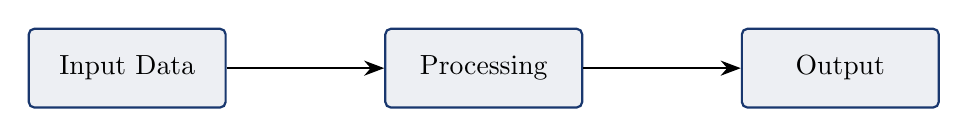
\begin{tikzpicture}[
        node distance=2cm,
        box/.style={rectangle, draw=linkcolor, fill=linkcolor!8, thick,
                    minimum width=2.5cm, minimum height=1cm, align=center, rounded corners=2pt},
        arrow/.style={-{Stealth[scale=1.1]}, thick}
    ]
        \node[box] (input) {Input Data};
        \node[box, right=of input] (process) {Processing};
        \node[box, right=of process] (output) {Output};
        \draw[arrow] (input) -- (process);
        \draw[arrow] (process) -- (output);
    \end{tikzpicture}
    \caption{A simple TikZ flowchart.}
    \label{fig:tikz}
\end{figure}

\chapter{Conclusion}
\label{ch:conclusion}

Summarize here.

% --- Bibliography ---
\bibliographystyle{plain}
\bibliography{references}

\end{document}
